% Graphic for TeX using PGF
% Title: C:\Users\Nicolas Chicaiza\Sourcetree\Metodología de la Investigación\Enfoque Marco Lógico\Esquemas\Árbol de Objetivos\arbolObjetivos.dia
% Creator: Dia v0.97.2
% CreationDate: Mon May 03 10:34:21 2021
% For: Nicolas Chicaiza
% \usepackage{tikz}
% The following commands are not supported in PSTricks at present
% We define them conditionally, so when they are implemented,
% this pgf file will use them.
\begin{figure}[H]
    \centering
    \ifx\du\undefined
    \newlength{\du}
    \fi
    \setlength{\du}{15\unitlength}
    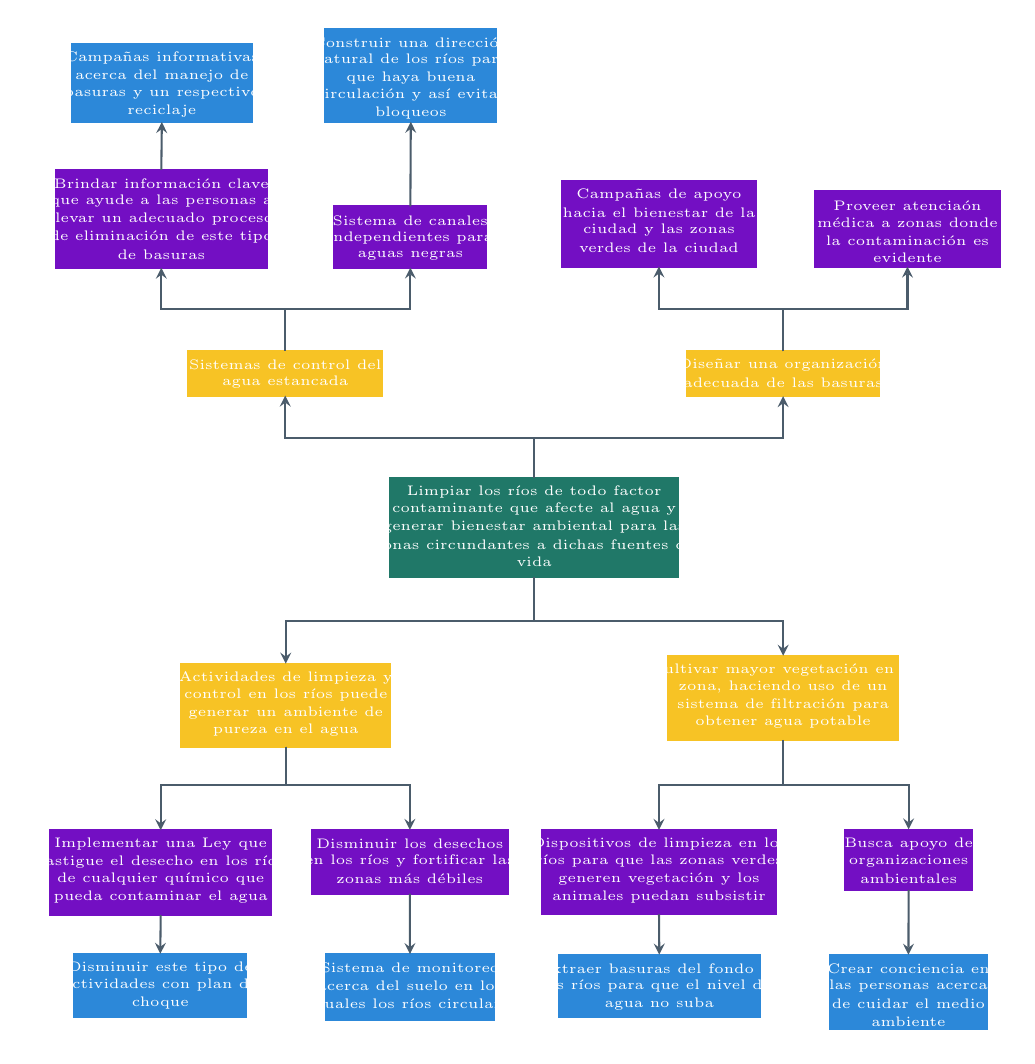
\begin{tikzpicture}[font = \tiny,every node/.style = {text = white}]
        \pgftransformxscale{1.000000}
        \pgftransformyscale{-1.000000}
        \definecolor{dialinecolor}{rgb}{0.000000, 0.000000, 0.000000}
        \pgfsetstrokecolor{dialinecolor}
        \definecolor{dialinecolor}{rgb}{1.000000, 1.000000, 1.000000}
        \pgfsetfillcolor{dialinecolor}
        \pgfsetlinewidth{0.050000\du}
        \pgfsetdash{}{0pt}
        \pgfsetdash{}{0pt}
        \pgfsetmiterjoin
        \definecolor{dialinecolor}{rgb}{0.125490, 0.470588, 0.407843}
        \pgfsetfillcolor{dialinecolor}
        \fill (-3.465863\du,-12.447222\du)--(-3.465863\du,-10.052251\du)--(3.475213\du,-10.052251\du)--(3.475213\du,-12.447222\du)--cycle;
        \definecolor{dialinecolor}{rgb}{0.125490, 0.470588, 0.407843}
        \pgfsetstrokecolor{dialinecolor}
        \draw (-3.465863\du,-12.447222\du)--(-3.465863\du,-10.052251\du)--(3.475213\du,-10.052251\du)--(3.475213\du,-12.447222\du)--cycle;
        % setfont left to latex
        \definecolor{dialinecolor}{rgb}{1.000000, 1.000000, 1.000000}
        \pgfsetstrokecolor{dialinecolor}
        \node at (0.004675\du,-12.109722\du){Limpiar los ríos de todo factor};
        % setfont left to latex
        \definecolor{dialinecolor}{rgb}{1.000000, 1.000000, 1.000000}
        \pgfsetstrokecolor{dialinecolor}
        \node at (0.004675\du,-11.686388\du){contaminante que afecte al agua y};
        % setfont left to latex
        \definecolor{dialinecolor}{rgb}{1.000000, 1.000000, 1.000000}
        \pgfsetstrokecolor{dialinecolor}
        \node at (0.004675\du,-11.263055\du){generar bienestar ambiental para las};
        % setfont left to latex
        \definecolor{dialinecolor}{rgb}{1.000000, 1.000000, 1.000000}
        \pgfsetstrokecolor{dialinecolor}
        \node at (0.004675\du,-10.839722\du){zonas circundantes a dichas fuentes de};
        % setfont left to latex
        \definecolor{dialinecolor}{rgb}{1.000000, 1.000000, 1.000000}
        \pgfsetstrokecolor{dialinecolor}
        \node at (0.004675\du,-10.416388\du){vida};
        \pgfsetlinewidth{0.050000\du}
        \pgfsetdash{}{0pt}
        \pgfsetdash{}{0pt}
        \pgfsetmiterjoin
        \definecolor{dialinecolor}{rgb}{0.968627, 0.764706, 0.145098}
        \pgfsetfillcolor{dialinecolor}
        \fill (-8.501116\du,-7.969845\du)--(-8.501116\du,-5.973226\du)--(-3.459108\du,-5.973226\du)--(-3.459108\du,-7.969845\du)--cycle;
        \definecolor{dialinecolor}{rgb}{0.968627, 0.764706, 0.145098}
        \pgfsetstrokecolor{dialinecolor}
        \draw (-8.501116\du,-7.969845\du)--(-8.501116\du,-5.973226\du)--(-3.459108\du,-5.973226\du)--(-3.459108\du,-7.969845\du)--cycle;
        % setfont left to latex
        \definecolor{dialinecolor}{rgb}{1.000000, 1.000000, 1.000000}
        \pgfsetstrokecolor{dialinecolor}
        \node at (-5.980112\du,-7.632345\du){Actividades de limpieza y};
        % setfont left to latex
        \definecolor{dialinecolor}{rgb}{1.000000, 1.000000, 1.000000}
        \pgfsetstrokecolor{dialinecolor}
        \node at (-5.980112\du,-7.209012\du){control en los ríos puede};
        % setfont left to latex
        \definecolor{dialinecolor}{rgb}{1.000000, 1.000000, 1.000000}
        \pgfsetstrokecolor{dialinecolor}
        \node at (-5.980112\du,-6.785678\du){generar un ambiente de};
        % setfont left to latex
        \definecolor{dialinecolor}{rgb}{1.000000, 1.000000, 1.000000}
        \pgfsetstrokecolor{dialinecolor}
        \node at (-5.980112\du,-6.362345\du){pureza en el agua};
        \pgfsetlinewidth{0.050000\du}
        \pgfsetdash{}{0pt}
        \pgfsetdash{}{0pt}
        \pgfsetmiterjoin
        \pgfsetbuttcap
        {
        \definecolor{dialinecolor}{rgb}{0.294118, 0.360784, 0.419608}
        \pgfsetfillcolor{dialinecolor}
        % was here!!!
        \pgfsetarrowsend{stealth}
        {\pgfsetcornersarced{\pgfpoint{0.000000\du}{0.000000\du}}\definecolor{dialinecolor}{rgb}{0.294118, 0.360784, 0.419608}
        \pgfsetstrokecolor{dialinecolor}
        \draw (0.004675\du,-10.052251\du)--(0.004675\du,-9.005283\du)--(-5.980112\du,-9.005283\du)--(-5.980112\du,-7.969845\du);
        }}
        \pgfsetlinewidth{0.050000\du}
        \pgfsetdash{}{0pt}
        \pgfsetdash{}{0pt}
        \pgfsetmiterjoin
        \definecolor{dialinecolor}{rgb}{0.968627, 0.764706, 0.145098}
        \pgfsetfillcolor{dialinecolor}
        \fill (3.226216\du,-8.160247\du)--(3.226216\du,-6.121584\du)--(8.776870\du,-6.121584\du)--(8.776870\du,-8.160247\du)--cycle;
        \definecolor{dialinecolor}{rgb}{0.968627, 0.764706, 0.145098}
        \pgfsetstrokecolor{dialinecolor}
        \draw (3.226216\du,-8.160247\du)--(3.226216\du,-6.121584\du)--(8.776870\du,-6.121584\du)--(8.776870\du,-8.160247\du)--cycle;
        % setfont left to latex
        \definecolor{dialinecolor}{rgb}{1.000000, 1.000000, 1.000000}
        \pgfsetstrokecolor{dialinecolor}
        \node at (6.001543\du,-7.822747\du){Cultivar mayor vegetación en la};
        % setfont left to latex
        \definecolor{dialinecolor}{rgb}{1.000000, 1.000000, 1.000000}
        \pgfsetstrokecolor{dialinecolor}
        \node at (6.001543\du,-7.399414\du){zona, haciendo uso de un};
        % setfont left to latex
        \definecolor{dialinecolor}{rgb}{1.000000, 1.000000, 1.000000}
        \pgfsetstrokecolor{dialinecolor}
        \node at (6.001543\du,-6.976081\du){sistema de filtración para};
        % setfont left to latex
        \definecolor{dialinecolor}{rgb}{1.000000, 1.000000, 1.000000}
        \pgfsetstrokecolor{dialinecolor}
        \node at (6.001543\du,-6.552747\du){obtener agua potable};
        \pgfsetlinewidth{0.050000\du}
        \pgfsetdash{}{0pt}
        \pgfsetdash{}{0pt}
        \pgfsetmiterjoin
        \pgfsetbuttcap
        {
        \definecolor{dialinecolor}{rgb}{0.294118, 0.360784, 0.419608}
        \pgfsetfillcolor{dialinecolor}
        % was here!!!
        \pgfsetarrowsend{stealth}
        {\pgfsetcornersarced{\pgfpoint{0.000000\du}{0.000000\du}}\definecolor{dialinecolor}{rgb}{0.294118, 0.360784, 0.419608}
        \pgfsetstrokecolor{dialinecolor}
        \draw (0.004675\du,-10.052251\du)--(0.004675\du,-9.002253\du)--(6.001543\du,-9.002253\du)--(6.001543\du,-8.160247\du);
        }}
        \pgfsetlinewidth{0.050000\du}
        \pgfsetdash{}{0pt}
        \pgfsetdash{}{0pt}
        \pgfsetmiterjoin
        \definecolor{dialinecolor}{rgb}{0.968627, 0.764706, 0.145098}
        \pgfsetfillcolor{dialinecolor}
        \fill (-8.324370\du,-15.507031\du)--(-8.324370\du,-14.427426\du)--(-3.659600\du,-14.427426\du)--(-3.659600\du,-15.507031\du)--cycle;
        \definecolor{dialinecolor}{rgb}{0.968627, 0.764706, 0.145098}
        \pgfsetstrokecolor{dialinecolor}
        \draw (-8.324370\du,-15.507031\du)--(-8.324370\du,-14.427426\du)--(-3.659600\du,-14.427426\du)--(-3.659600\du,-15.507031\du)--cycle;
        % setfont left to latex
        \definecolor{dialinecolor}{rgb}{1.000000, 1.000000, 1.000000}
        \pgfsetstrokecolor{dialinecolor}
        \node at (-5.991985\du,-15.169531\du){Sistemas de control del};
        % setfont left to latex
        \definecolor{dialinecolor}{rgb}{1.000000, 1.000000, 1.000000}
        \pgfsetstrokecolor{dialinecolor}
        \node at (-5.991985\du,-14.746197\du){agua estancada};
        \pgfsetlinewidth{0.050000\du}
        \pgfsetdash{}{0pt}
        \pgfsetdash{}{0pt}
        \pgfsetmiterjoin
        \pgfsetbuttcap
        {
        \definecolor{dialinecolor}{rgb}{0.294118, 0.360784, 0.419608}
        \pgfsetfillcolor{dialinecolor}
        % was here!!!
        \pgfsetarrowsend{stealth}
        {\pgfsetcornersarced{\pgfpoint{0.000000\du}{0.000000\du}}\definecolor{dialinecolor}{rgb}{0.294118, 0.360784, 0.419608}
        \pgfsetstrokecolor{dialinecolor}
        \draw (0.004675\du,-12.447222\du)--(0.004675\du,-13.411507\du)--(-5.991985\du,-13.411507\du)--(-5.991985\du,-14.427426\du);
        }}
        \pgfsetlinewidth{0.050000\du}
        \pgfsetdash{}{0pt}
        \pgfsetdash{}{0pt}
        \pgfsetmiterjoin
        \definecolor{dialinecolor}{rgb}{0.968627, 0.764706, 0.145098}
        \pgfsetfillcolor{dialinecolor}
        \fill (3.692105\du,-15.493259\du)--(3.692105\du,-14.413655\du)--(8.311009\du,-14.413655\du)--(8.311009\du,-15.493259\du)--cycle;
        \definecolor{dialinecolor}{rgb}{0.968627, 0.764706, 0.145098}
        \pgfsetstrokecolor{dialinecolor}
        \draw (3.692105\du,-15.493259\du)--(3.692105\du,-14.413655\du)--(8.311009\du,-14.413655\du)--(8.311009\du,-15.493259\du)--cycle;
        % setfont left to latex
        \definecolor{dialinecolor}{rgb}{1.000000, 1.000000, 1.000000}
        \pgfsetstrokecolor{dialinecolor}
        \node at (6.001557\du,-15.155759\du){Diseñar una organización};
        % setfont left to latex
        \definecolor{dialinecolor}{rgb}{1.000000, 1.000000, 1.000000}
        \pgfsetstrokecolor{dialinecolor}
        \node at (6.001557\du,-14.732426\du){adecuada de las basuras};
        \pgfsetlinewidth{0.050000\du}
        \pgfsetdash{}{0pt}
        \pgfsetdash{}{0pt}
        \pgfsetmiterjoin
        \pgfsetbuttcap
        {
        \definecolor{dialinecolor}{rgb}{0.294118, 0.360784, 0.419608}
        \pgfsetfillcolor{dialinecolor}
        % was here!!!
        \pgfsetarrowsend{stealth}
        {\pgfsetcornersarced{\pgfpoint{0.000000\du}{0.000000\du}}\definecolor{dialinecolor}{rgb}{0.294118, 0.360784, 0.419608}
        \pgfsetstrokecolor{dialinecolor}
        \draw (0.004675\du,-12.447222\du)--(0.004675\du,-13.412893\du)--(6.001557\du,-13.412893\du)--(6.001557\du,-14.413655\du);
        }}
        \pgfsetlinewidth{0.050000\du}
        \pgfsetdash{}{0pt}
        \pgfsetdash{}{0pt}
        \pgfsetmiterjoin
        \definecolor{dialinecolor}{rgb}{0.450980, 0.058824, 0.764706}
        \pgfsetfillcolor{dialinecolor}
        \fill (-11.658277\du,-3.955003\du)--(-11.658277\du,-1.909814\du)--(-6.327921\du,-1.909814\du)--(-6.327921\du,-3.955003\du)--cycle;
        \definecolor{dialinecolor}{rgb}{0.450980, 0.058824, 0.764706}
        \pgfsetstrokecolor{dialinecolor}
        \draw (-11.658277\du,-3.955003\du)--(-11.658277\du,-1.909814\du)--(-6.327921\du,-1.909814\du)--(-6.327921\du,-3.955003\du)--cycle;
        % setfont left to latex
        \definecolor{dialinecolor}{rgb}{1.000000, 1.000000, 1.000000}
        \pgfsetstrokecolor{dialinecolor}
        \node at (-8.993099\du,-3.617503\du){Implementar una Ley que};
        % setfont left to latex
        \definecolor{dialinecolor}{rgb}{1.000000, 1.000000, 1.000000}
        \pgfsetstrokecolor{dialinecolor}
        \node at (-8.993099\du,-3.194169\du){ castigue el desecho en los ríos};
        % setfont left to latex
        \definecolor{dialinecolor}{rgb}{1.000000, 1.000000, 1.000000}
        \pgfsetstrokecolor{dialinecolor}
        \node at (-8.993099\du,-2.770836\du){de cualquier químico que};
        % setfont left to latex
        \definecolor{dialinecolor}{rgb}{1.000000, 1.000000, 1.000000}
        \pgfsetstrokecolor{dialinecolor}
        \node at (-8.993099\du,-2.347503\du){pueda contaminar el agua};
        \pgfsetlinewidth{0.050000\du}
        \pgfsetdash{}{0pt}
        \pgfsetdash{}{0pt}
        \pgfsetmiterjoin
        \pgfsetbuttcap
        {
        \definecolor{dialinecolor}{rgb}{0.294118, 0.360784, 0.419608}
        \pgfsetfillcolor{dialinecolor}
        % was here!!!
        \pgfsetarrowsend{stealth}
        {\pgfsetcornersarced{\pgfpoint{0.000000\du}{0.000000\du}}\definecolor{dialinecolor}{rgb}{0.294118, 0.360784, 0.419608}
        \pgfsetstrokecolor{dialinecolor}
        \draw (-5.980112\du,-5.973226\du)--(-5.980112\du,-5.048256\du)--(-8.993099\du,-5.048256\du)--(-8.993099\du,-3.955003\du);
        }}
        \pgfsetlinewidth{0.050000\du}
        \pgfsetdash{}{0pt}
        \pgfsetdash{}{0pt}
        \pgfsetmiterjoin
        \definecolor{dialinecolor}{rgb}{0.450980, 0.058824, 0.764706}
        \pgfsetfillcolor{dialinecolor}
        \fill (-5.344005\du,-3.964767\du)--(-5.344005\du,-2.424107\du)--(-0.638023\du,-2.424107\du)--(-0.638023\du,-3.964767\du)--cycle;
        \definecolor{dialinecolor}{rgb}{0.450980, 0.058824, 0.764706}
        \pgfsetstrokecolor{dialinecolor}
        \draw (-5.344005\du,-3.964767\du)--(-5.344005\du,-2.424107\du)--(-0.638023\du,-2.424107\du)--(-0.638023\du,-3.964767\du)--cycle;
        % setfont left to latex
        \definecolor{dialinecolor}{rgb}{1.000000, 1.000000, 1.000000}
        \pgfsetstrokecolor{dialinecolor}
        \node at (-2.991014\du,-3.627267\du){Disminuir los desechos};
        % setfont left to latex
        \definecolor{dialinecolor}{rgb}{1.000000, 1.000000, 1.000000}
        \pgfsetstrokecolor{dialinecolor}
        \node at (-2.991014\du,-3.203934\du){en los ríos y fortificar las};
        % setfont left to latex
        \definecolor{dialinecolor}{rgb}{1.000000, 1.000000, 1.000000}
        \pgfsetstrokecolor{dialinecolor}
        \node at (-2.991014\du,-2.780600\du){zonas más débiles};
        \pgfsetlinewidth{0.050000\du}
        \pgfsetdash{}{0pt}
        \pgfsetdash{}{0pt}
        \pgfsetmiterjoin
        \pgfsetbuttcap
        {
        \definecolor{dialinecolor}{rgb}{0.294118, 0.360784, 0.419608}
        \pgfsetfillcolor{dialinecolor}
        % was here!!!
        \pgfsetarrowsend{stealth}
        {\pgfsetcornersarced{\pgfpoint{0.000000\du}{0.000000\du}}\definecolor{dialinecolor}{rgb}{0.294118, 0.360784, 0.419608}
        \pgfsetstrokecolor{dialinecolor}
        \draw (-5.980112\du,-5.973226\du)--(-5.980112\du,-5.048256\du)--(-2.991014\du,-5.048256\du)--(-2.991014\du,-3.964767\du);
        }}
        \pgfsetlinewidth{0.050000\du}
        \pgfsetdash{}{0pt}
        \pgfsetdash{}{0pt}
        \pgfsetmiterjoin
        \definecolor{dialinecolor}{rgb}{0.172549, 0.533333, 0.850980}
        \pgfsetfillcolor{dialinecolor}
        \fill (-11.069660\du,-0.979973\du)--(-11.069660\du,0.543608\du)--(-6.937061\du,0.543608\du)--(-6.937061\du,-0.979973\du)--cycle;
        \definecolor{dialinecolor}{rgb}{0.172549, 0.533333, 0.850980}
        \pgfsetstrokecolor{dialinecolor}
        \draw (-11.069660\du,-0.979973\du)--(-11.069660\du,0.543608\du)--(-6.937061\du,0.543608\du)--(-6.937061\du,-0.979973\du)--cycle;
        \pgfsetlinewidth{0.050000\du}
        \pgfsetdash{}{0pt}
        \pgfsetdash{}{0pt}
        \pgfsetbuttcap
        {
        \definecolor{dialinecolor}{rgb}{0.294118, 0.360784, 0.419608}
        \pgfsetfillcolor{dialinecolor}
        % was here!!!
        \pgfsetarrowsend{stealth}
        \definecolor{dialinecolor}{rgb}{0.294118, 0.360784, 0.419608}
        \pgfsetstrokecolor{dialinecolor}
        \draw (-8.993099\du,-1.909814\du)--(-9.003360\du,-0.979973\du);
        }
        % setfont left to latex
        \definecolor{dialinecolor}{rgb}{1.000000, 1.000000, 1.000000}
        \pgfsetstrokecolor{dialinecolor}
        \node at (-9.003360\du,-0.642473\du){Disminuir este tipo de};
        % setfont left to latex
        \definecolor{dialinecolor}{rgb}{1.000000, 1.000000, 1.000000}
        \pgfsetstrokecolor{dialinecolor}
        \node at (-9.003360\du,-0.219140\du){actividades con plan de};
        % setfont left to latex
        \definecolor{dialinecolor}{rgb}{1.000000, 1.000000, 1.000000}
        \pgfsetstrokecolor{dialinecolor}
        \node at (-9.003360\du,0.204193\du){choque};
        \pgfsetlinewidth{0.050000\du}
        \pgfsetdash{}{0pt}
        \pgfsetdash{}{0pt}
        \pgfsetmiterjoin
        \definecolor{dialinecolor}{rgb}{0.172549, 0.533333, 0.850980}
        \pgfsetfillcolor{dialinecolor}
        \fill (-5.008887\du,-0.973416\du)--(-5.008887\du,0.623892\du)--(-0.968178\du,0.623892\du)--(-0.968178\du,-0.973416\du)--cycle;
        \definecolor{dialinecolor}{rgb}{0.172549, 0.533333, 0.850980}
        \pgfsetstrokecolor{dialinecolor}
        \draw (-5.008887\du,-0.973416\du)--(-5.008887\du,0.623892\du)--(-0.968178\du,0.623892\du)--(-0.968178\du,-0.973416\du)--cycle;
        % setfont left to latex
        \definecolor{dialinecolor}{rgb}{1.000000, 1.000000, 1.000000}
        \pgfsetstrokecolor{dialinecolor}
        \node at (-2.988532\du,-0.635916\du){Sistema de monitoreo};
        % setfont left to latex
        \definecolor{dialinecolor}{rgb}{1.000000, 1.000000, 1.000000}
        \pgfsetstrokecolor{dialinecolor}
        \node at (-2.988532\du,-0.212583\du){acerca del suelo en los};
        % setfont left to latex
        \definecolor{dialinecolor}{rgb}{1.000000, 1.000000, 1.000000}
        \pgfsetstrokecolor{dialinecolor}
        \node at (-2.988532\du,0.210751\du){cuales los ríos circulan};
        \pgfsetlinewidth{0.050000\du}
        \pgfsetdash{}{0pt}
        \pgfsetdash{}{0pt}
        \pgfsetbuttcap
        {
        \definecolor{dialinecolor}{rgb}{0.294118, 0.360784, 0.419608}
        \pgfsetfillcolor{dialinecolor}
        % was here!!!
        \pgfsetarrowsend{stealth}
        \definecolor{dialinecolor}{rgb}{0.294118, 0.360784, 0.419608}
        \pgfsetstrokecolor{dialinecolor}
        \draw (-2.991014\du,-2.424107\du)--(-2.988532\du,-0.973416\du);
        }
        \pgfsetlinewidth{0.050000\du}
        \pgfsetdash{}{0pt}
        \pgfsetdash{}{0pt}
        \pgfsetmiterjoin
        \definecolor{dialinecolor}{rgb}{0.450980, 0.058824, 0.764706}
        \pgfsetfillcolor{dialinecolor}
        \fill (-11.518357\du,-19.862893\du)--(-11.518357\du,-17.509268\du)--(-6.438253\du,-17.509268\du)--(-6.438253\du,-19.862893\du)--cycle;
        \definecolor{dialinecolor}{rgb}{0.450980, 0.058824, 0.764706}
        \pgfsetstrokecolor{dialinecolor}
        \draw (-11.518357\du,-19.862893\du)--(-11.518357\du,-17.509268\du)--(-6.438253\du,-17.509268\du)--(-6.438253\du,-19.862893\du)--cycle;
        % setfont left to latex
        \definecolor{dialinecolor}{rgb}{1.000000, 1.000000, 1.000000}
        \pgfsetstrokecolor{dialinecolor}
        \node at (-8.978305\du,-19.525393\du){Brindar información clave};
        % setfont left to latex
        \definecolor{dialinecolor}{rgb}{1.000000, 1.000000, 1.000000}
        \pgfsetstrokecolor{dialinecolor}
        \node at (-8.978305\du,-19.102060\du){que ayude a las personas a};
        % setfont left to latex
        \definecolor{dialinecolor}{rgb}{1.000000, 1.000000, 1.000000}
        \pgfsetstrokecolor{dialinecolor}
        \node at (-8.978305\du,-18.678727\du){llevar un adecuado proceso};
        % setfont left to latex
        \definecolor{dialinecolor}{rgb}{1.000000, 1.000000, 1.000000}
        \pgfsetstrokecolor{dialinecolor}
        \node at (-8.978305\du,-18.255393\du){de eliminación de este tipo};
        % setfont left to latex
        \definecolor{dialinecolor}{rgb}{1.000000, 1.000000, 1.000000}
        \pgfsetstrokecolor{dialinecolor}
        \node at (-8.978305\du,-17.832060\du){de basuras};
        \pgfsetlinewidth{0.050000\du}
        \pgfsetdash{}{0pt}
        \pgfsetdash{}{0pt}
        \pgfsetmiterjoin
        \pgfsetbuttcap
        {
        \definecolor{dialinecolor}{rgb}{0.294118, 0.360784, 0.419608}
        \pgfsetfillcolor{dialinecolor}
        % was here!!!
        \pgfsetarrowsend{stealth}
        {\pgfsetcornersarced{\pgfpoint{0.000000\du}{0.000000\du}}\definecolor{dialinecolor}{rgb}{0.294118, 0.360784, 0.419608}
        \pgfsetstrokecolor{dialinecolor}
        \draw (-5.991985\du,-15.507031\du)--(-5.991985\du,-16.508149\du)--(-8.978305\du,-16.508149\du)--(-8.978305\du,-17.509268\du);
        }}
        \pgfsetlinewidth{0.050000\du}
        \pgfsetdash{}{0pt}
        \pgfsetdash{}{0pt}
        \pgfsetmiterjoin
        \definecolor{dialinecolor}{rgb}{0.450980, 0.058824, 0.764706}
        \pgfsetfillcolor{dialinecolor}
        \fill (-4.807224\du,-18.982429\du)--(-4.807224\du,-17.511729\du)--(-1.150332\du,-17.511729\du)--(-1.150332\du,-18.982429\du)--cycle;
        \definecolor{dialinecolor}{rgb}{0.450980, 0.058824, 0.764706}
        \pgfsetstrokecolor{dialinecolor}
        \draw (-4.807224\du,-18.982429\du)--(-4.807224\du,-17.511729\du)--(-1.150332\du,-17.511729\du)--(-1.150332\du,-18.982429\du)--cycle;
        % setfont left to latex
        \definecolor{dialinecolor}{rgb}{1.000000, 1.000000, 1.000000}
        \pgfsetstrokecolor{dialinecolor}
        \node at (-2.978778\du,-18.644929\du){Sistema de canales};
        % setfont left to latex
        \definecolor{dialinecolor}{rgb}{1.000000, 1.000000, 1.000000}
        \pgfsetstrokecolor{dialinecolor}
        \node at (-2.978778\du,-18.221596\du){independientes para};
        % setfont left to latex
        \definecolor{dialinecolor}{rgb}{1.000000, 1.000000, 1.000000}
        \pgfsetstrokecolor{dialinecolor}
        \node at (-2.978778\du,-17.798263\du){aguas negras};
        \pgfsetlinewidth{0.050000\du}
        \pgfsetdash{}{0pt}
        \pgfsetdash{}{0pt}
        \pgfsetmiterjoin
        \pgfsetbuttcap
        {
        \definecolor{dialinecolor}{rgb}{0.294118, 0.360784, 0.419608}
        \pgfsetfillcolor{dialinecolor}
        % was here!!!
        \pgfsetarrowsend{stealth}
        {\pgfsetcornersarced{\pgfpoint{0.000000\du}{0.000000\du}}\definecolor{dialinecolor}{rgb}{0.294118, 0.360784, 0.419608}
        \pgfsetstrokecolor{dialinecolor}
        \draw (-5.991985\du,-15.507031\du)--(-5.991985\du,-16.509380\du)--(-2.978778\du,-16.509380\du)--(-2.978778\du,-17.511729\du);
        }}
        \pgfsetlinewidth{0.050000\du}
        \pgfsetdash{}{0pt}
        \pgfsetdash{}{0pt}
        \pgfsetmiterjoin
        \definecolor{dialinecolor}{rgb}{0.172549, 0.533333, 0.850980}
        \pgfsetfillcolor{dialinecolor}
        \fill (-11.129385\du,-22.891523\du)--(-11.129385\du,-21.017460\du)--(-6.802329\du,-21.017460\du)--(-6.802329\du,-22.891523\du)--cycle;
        \definecolor{dialinecolor}{rgb}{0.172549, 0.533333, 0.850980}
        \pgfsetstrokecolor{dialinecolor}
        \draw (-11.129385\du,-22.891523\du)--(-11.129385\du,-21.017460\du)--(-6.802329\du,-21.017460\du)--(-6.802329\du,-22.891523\du)--cycle;
        \pgfsetlinewidth{0.050000\du}
        \pgfsetdash{}{0pt}
        \pgfsetdash{}{0pt}
        \pgfsetbuttcap
        {
        \definecolor{dialinecolor}{rgb}{0.294118, 0.360784, 0.419608}
        \pgfsetfillcolor{dialinecolor}
        % was here!!!
        \pgfsetarrowsend{stealth}
        \definecolor{dialinecolor}{rgb}{0.294118, 0.360784, 0.419608}
        \pgfsetstrokecolor{dialinecolor}
        \draw (-8.978305\du,-19.862893\du)--(-8.965857\du,-21.017460\du);
        }
        % setfont left to latex
        \definecolor{dialinecolor}{rgb}{1.000000, 1.000000, 1.000000}
        \pgfsetstrokecolor{dialinecolor}
        \node at (-8.965857\du,-22.554023\du){Campañas informativas};
        % setfont left to latex
        \definecolor{dialinecolor}{rgb}{1.000000, 1.000000, 1.000000}
        \pgfsetstrokecolor{dialinecolor}
        \node at (-8.965857\du,-22.130690\du){acerca del manejo de};
        % setfont left to latex
        \definecolor{dialinecolor}{rgb}{1.000000, 1.000000, 1.000000}
        \pgfsetstrokecolor{dialinecolor}
        \node at (-8.965857\du,-21.707356\du){basuras y un respectivo};
        % setfont left to latex
        \definecolor{dialinecolor}{rgb}{1.000000, 1.000000, 1.000000}
        \pgfsetstrokecolor{dialinecolor}
        \node at (-8.965857\du,-21.284023\du){reciclaje};
        \pgfsetlinewidth{0.050000\du}
        \pgfsetdash{}{0pt}
        \pgfsetdash{}{0pt}
        \pgfsetmiterjoin
        \definecolor{dialinecolor}{rgb}{0.172549, 0.533333, 0.850980}
        \pgfsetfillcolor{dialinecolor}
        \fill (-5.031775\du,-23.265418\du)--(-5.031775\du,-21.023320\du)--(-0.904967\du,-21.023320\du)--(-0.904967\du,-23.265418\du)--cycle;
        \definecolor{dialinecolor}{rgb}{0.172549, 0.533333, 0.850980}
        \pgfsetstrokecolor{dialinecolor}
        \draw (-5.031775\du,-23.265418\du)--(-5.031775\du,-21.023320\du)--(-0.904967\du,-21.023320\du)--(-0.904967\du,-23.265418\du)--cycle;
        % setfont left to latex
        \definecolor{dialinecolor}{rgb}{1.000000, 1.000000, 1.000000}
        \pgfsetstrokecolor{dialinecolor}
        \node at (-2.968371\du,-22.927918\du){Construir una dirección};
        % setfont left to latex
        \definecolor{dialinecolor}{rgb}{1.000000, 1.000000, 1.000000}
        \pgfsetstrokecolor{dialinecolor}
        \node at (-2.968371\du,-22.504585\du){natural de los ríos para};
        % setfont left to latex
        \definecolor{dialinecolor}{rgb}{1.000000, 1.000000, 1.000000}
        \pgfsetstrokecolor{dialinecolor}
        \node at (-2.968371\du,-22.081252\du){que haya buena};
        % setfont left to latex
        \definecolor{dialinecolor}{rgb}{1.000000, 1.000000, 1.000000}
        \pgfsetstrokecolor{dialinecolor}
        \node at (-2.968371\du,-21.657918\du){circulación y así evitar};
        % setfont left to latex
        \definecolor{dialinecolor}{rgb}{1.000000, 1.000000, 1.000000}
        \pgfsetstrokecolor{dialinecolor}
        \node at (-2.968371\du,-21.234585\du){bloqueos};
        \pgfsetlinewidth{0.050000\du}
        \pgfsetdash{}{0pt}
        \pgfsetdash{}{0pt}
        \pgfsetbuttcap
        {
        \definecolor{dialinecolor}{rgb}{0.294118, 0.360784, 0.419608}
        \pgfsetfillcolor{dialinecolor}
        % was here!!!
        \pgfsetarrowsend{stealth}
        \definecolor{dialinecolor}{rgb}{0.294118, 0.360784, 0.419608}
        \pgfsetstrokecolor{dialinecolor}
        \draw (-2.978778\du,-18.982429\du)--(-2.968371\du,-21.023320\du);
        }
        \pgfsetlinewidth{0.050000\du}
        \pgfsetdash{}{0pt}
        \pgfsetdash{}{0pt}
        \pgfsetmiterjoin
        \definecolor{dialinecolor}{rgb}{0.450980, 0.058824, 0.764706}
        \pgfsetfillcolor{dialinecolor}
        \fill (0.681751\du,-19.604648\du)--(0.681751\du,-17.537320\du)--(5.338016\du,-17.537320\du)--(5.338016\du,-19.604648\du)--cycle;
        \definecolor{dialinecolor}{rgb}{0.450980, 0.058824, 0.764706}
        \pgfsetstrokecolor{dialinecolor}
        \draw (0.681751\du,-19.604648\du)--(0.681751\du,-17.537320\du)--(5.338016\du,-17.537320\du)--(5.338016\du,-19.604648\du)--cycle;
        % setfont left to latex
        \definecolor{dialinecolor}{rgb}{1.000000, 1.000000, 1.000000}
        \pgfsetstrokecolor{dialinecolor}
        \node at (3.009884\du,-19.267148\du){Campañas de apoyo};
        % setfont left to latex
        \definecolor{dialinecolor}{rgb}{1.000000, 1.000000, 1.000000}
        \pgfsetstrokecolor{dialinecolor}
        \node at (3.009884\du,-18.843815\du){hacia el bienestar de la};
        % setfont left to latex
        \definecolor{dialinecolor}{rgb}{1.000000, 1.000000, 1.000000}
        \pgfsetstrokecolor{dialinecolor}
        \node at (3.009884\du,-18.420482\du){ciudad y las zonas};
        % setfont left to latex
        \definecolor{dialinecolor}{rgb}{1.000000, 1.000000, 1.000000}
        \pgfsetstrokecolor{dialinecolor}
        \node at (3.009884\du,-17.997148\du){verdes de la ciudad};
        \pgfsetlinewidth{0.050000\du}
        \pgfsetdash{}{0pt}
        \pgfsetdash{}{0pt}
        \pgfsetmiterjoin
        \pgfsetbuttcap
        {
        \definecolor{dialinecolor}{rgb}{0.294118, 0.360784, 0.419608}
        \pgfsetfillcolor{dialinecolor}
        % was here!!!
        \pgfsetarrowsend{stealth}
        {\pgfsetcornersarced{\pgfpoint{0.000000\du}{0.000000\du}}\definecolor{dialinecolor}{rgb}{0.294118, 0.360784, 0.419608}
        \pgfsetstrokecolor{dialinecolor}
        \draw (6.001557\du,-15.493259\du)--(6.001557\du,-16.515290\du)--(3.009884\du,-16.515290\du)--(3.009884\du,-17.537320\du);
        }}
        \pgfsetlinewidth{0.050000\du}
        \pgfsetdash{}{0pt}
        \pgfsetdash{}{0pt}
        \pgfsetmiterjoin
        \definecolor{dialinecolor}{rgb}{0.450980, 0.058824, 0.764706}
        \pgfsetfillcolor{dialinecolor}
        \fill (6.770279\du,-19.350438\du)--(6.770279\du,-17.535375\du)--(11.222612\du,-17.535375\du)--(11.222612\du,-19.350438\du)--cycle;
        \definecolor{dialinecolor}{rgb}{0.450980, 0.058824, 0.764706}
        \pgfsetstrokecolor{dialinecolor}
        \draw (6.770279\du,-19.350438\du)--(6.770279\du,-17.535375\du)--(11.222612\du,-17.535375\du)--(11.222612\du,-19.350438\du)--cycle;
        % setfont left to latex
        \definecolor{dialinecolor}{rgb}{1.000000, 1.000000, 1.000000}
        \pgfsetstrokecolor{dialinecolor}
        \node at (8.996446\du,-19.012938\du){Proveer atenciaón};
        % setfont left to latex
        \definecolor{dialinecolor}{rgb}{1.000000, 1.000000, 1.000000}
        \pgfsetstrokecolor{dialinecolor}
        \node at (8.996446\du,-18.589605\du){médica a zonas donde};
        % setfont left to latex
        \definecolor{dialinecolor}{rgb}{1.000000, 1.000000, 1.000000}
        \pgfsetstrokecolor{dialinecolor}
        \node at (8.996446\du,-18.166271\du){la contaminación es};
        % setfont left to latex
        \definecolor{dialinecolor}{rgb}{1.000000, 1.000000, 1.000000}
        \pgfsetstrokecolor{dialinecolor}
        \node at (8.996446\du,-17.742938\du){evidente};
        \pgfsetlinewidth{0.050000\du}
        \pgfsetdash{}{0pt}
        \pgfsetdash{}{0pt}
        \pgfsetmiterjoin
        \pgfsetbuttcap
        {
        \definecolor{dialinecolor}{rgb}{0.294118, 0.360784, 0.419608}
        \pgfsetfillcolor{dialinecolor}
        % was here!!!
        \pgfsetarrowsend{stealth}
        {\pgfsetcornersarced{\pgfpoint{0.000000\du}{0.000000\du}}\definecolor{dialinecolor}{rgb}{0.294118, 0.360784, 0.419608}
        \pgfsetstrokecolor{dialinecolor}
        \draw (6.001557\du,-15.493259\du)--(6.001557\du,-16.514317\du)--(8.996446\du,-16.514317\du)--(8.996446\du,-17.535375\du);
        }}
        \pgfsetlinewidth{0.050000\du}
        \pgfsetdash{}{0pt}
        \pgfsetdash{}{0pt}
        \pgfsetmiterjoin
        \definecolor{dialinecolor}{rgb}{0.450980, 0.058824, 0.764706}
        \pgfsetfillcolor{dialinecolor}
        \fill (0.184686\du,-3.964689\du)--(0.184686\du,-1.930125\du)--(5.837712\du,-1.930125\du)--(5.837712\du,-3.964689\du)--cycle;
        \definecolor{dialinecolor}{rgb}{0.450980, 0.058824, 0.764706}
        \pgfsetstrokecolor{dialinecolor}
        \draw (0.184686\du,-3.964689\du)--(0.184686\du,-1.930125\du)--(5.837712\du,-1.930125\du)--(5.837712\du,-3.964689\du)--cycle;
        % setfont left to latex
        \definecolor{dialinecolor}{rgb}{1.000000, 1.000000, 1.000000}
        \pgfsetstrokecolor{dialinecolor}
        \node at (3.011199\du,-3.627189\du){Dispositivos de limpieza en los};
        % setfont left to latex
        \definecolor{dialinecolor}{rgb}{1.000000, 1.000000, 1.000000}
        \pgfsetstrokecolor{dialinecolor}
        \node at (3.011199\du,-3.203856\du){ríos para que las zonas verdes};
        % setfont left to latex
        \definecolor{dialinecolor}{rgb}{1.000000, 1.000000, 1.000000}
        \pgfsetstrokecolor{dialinecolor}
        \node at (3.011199\du,-2.780522\du){generen vegetación y los};
        % setfont left to latex
        \definecolor{dialinecolor}{rgb}{1.000000, 1.000000, 1.000000}
        \pgfsetstrokecolor{dialinecolor}
        \node at (3.011199\du,-2.357189\du){animales puedan subsistir};
        \pgfsetlinewidth{0.050000\du}
        \pgfsetdash{}{0pt}
        \pgfsetdash{}{0pt}
        \pgfsetmiterjoin
        \pgfsetbuttcap
        {
        \definecolor{dialinecolor}{rgb}{0.294118, 0.360784, 0.419608}
        \pgfsetfillcolor{dialinecolor}
        % was here!!!
        \pgfsetarrowsend{stealth}
        {\pgfsetcornersarced{\pgfpoint{0.000000\du}{0.000000\du}}\definecolor{dialinecolor}{rgb}{0.294118, 0.360784, 0.419608}
        \pgfsetstrokecolor{dialinecolor}
        \draw (6.001543\du,-6.121584\du)--(6.001543\du,-5.043137\du)--(3.011199\du,-5.043137\du)--(3.011199\du,-3.964689\du);
        }}
        \pgfsetlinewidth{0.050000\du}
        \pgfsetdash{}{0pt}
        \pgfsetdash{}{0pt}
        \pgfsetmiterjoin
        \definecolor{dialinecolor}{rgb}{0.450980, 0.058824, 0.764706}
        \pgfsetfillcolor{dialinecolor}
        \fill (7.497809\du,-3.964653\du)--(7.497809\du,-2.518706\du)--(10.550389\du,-2.518706\du)--(10.550389\du,-3.964653\du)--cycle;
        \definecolor{dialinecolor}{rgb}{0.450980, 0.058824, 0.764706}
        \pgfsetstrokecolor{dialinecolor}
        \draw (7.497809\du,-3.964653\du)--(7.497809\du,-2.518706\du)--(10.550389\du,-2.518706\du)--(10.550389\du,-3.964653\du)--cycle;
        % setfont left to latex
        \definecolor{dialinecolor}{rgb}{1.000000, 1.000000, 1.000000}
        \pgfsetstrokecolor{dialinecolor}
        \node at (9.024099\du,-3.627153\du){Busca apoyo de};
        % setfont left to latex
        \definecolor{dialinecolor}{rgb}{1.000000, 1.000000, 1.000000}
        \pgfsetstrokecolor{dialinecolor}
        \node at (9.024099\du,-3.203819\du){organizaciones};
        % setfont left to latex
        \definecolor{dialinecolor}{rgb}{1.000000, 1.000000, 1.000000}
        \pgfsetstrokecolor{dialinecolor}
        \node at (9.024099\du,-2.780486\du){ambientales};
        \pgfsetlinewidth{0.050000\du}
        \pgfsetdash{}{0pt}
        \pgfsetdash{}{0pt}
        \pgfsetmiterjoin
        \pgfsetbuttcap
        {
        \definecolor{dialinecolor}{rgb}{0.294118, 0.360784, 0.419608}
        \pgfsetfillcolor{dialinecolor}
        % was here!!!
        \pgfsetarrowsend{stealth}
        {\pgfsetcornersarced{\pgfpoint{0.000000\du}{0.000000\du}}\definecolor{dialinecolor}{rgb}{0.294118, 0.360784, 0.419608}
        \pgfsetstrokecolor{dialinecolor}
        \draw (6.001543\du,-6.133046\du)--(6.001543\du,-5.047021\du)--(9.024099\du,-5.047021\du)--(9.024099\du,-3.976114\du);
        }}
        \pgfsetlinewidth{0.050000\du}
        \pgfsetdash{}{0pt}
        \pgfsetdash{}{0pt}
        \pgfsetmiterjoin
        \definecolor{dialinecolor}{rgb}{0.172549, 0.533333, 0.850980}
        \pgfsetfillcolor{dialinecolor}
        \fill (0.602420\du,-0.960801\du)--(0.602420\du,0.552156\du)--(5.433150\du,0.552156\du)--(5.433150\du,-0.960801\du)--cycle;
        \definecolor{dialinecolor}{rgb}{0.172549, 0.533333, 0.850980}
        \pgfsetstrokecolor{dialinecolor}
        \draw (0.602420\du,-0.960801\du)--(0.602420\du,0.552156\du)--(5.433150\du,0.552156\du)--(5.433150\du,-0.960801\du)--cycle;
        \pgfsetlinewidth{0.050000\du}
        \pgfsetdash{}{0pt}
        \pgfsetdash{}{0pt}
        \pgfsetbuttcap
        {
        \definecolor{dialinecolor}{rgb}{0.294118, 0.360784, 0.419608}
        \pgfsetfillcolor{dialinecolor}
        % was here!!!
        \pgfsetarrowsend{stealth}
        \definecolor{dialinecolor}{rgb}{0.294118, 0.360784, 0.419608}
        \pgfsetstrokecolor{dialinecolor}
        \draw (3.011199\du,-1.930125\du)--(3.017785\du,-0.960801\du);
        }
        % setfont left to latex
        \definecolor{dialinecolor}{rgb}{1.000000, 1.000000, 1.000000}
        \pgfsetstrokecolor{dialinecolor}
        \node at (3.017785\du,-0.623301\du){Extraer basuras del fondo de};
        % setfont left to latex
        \definecolor{dialinecolor}{rgb}{1.000000, 1.000000, 1.000000}
        \pgfsetstrokecolor{dialinecolor}
        \node at (3.017785\du,-0.199968\du){los ríos para que el nivel del};
        % setfont left to latex
        \definecolor{dialinecolor}{rgb}{1.000000, 1.000000, 1.000000}
        \pgfsetstrokecolor{dialinecolor}
        \node at (3.017785\du,0.223366\du){agua no suba};
        \pgfsetlinewidth{0.050000\du}
        \pgfsetdash{}{0pt}
        \pgfsetdash{}{0pt}
        \pgfsetmiterjoin
        \definecolor{dialinecolor}{rgb}{0.172549, 0.533333, 0.850980}
        \pgfsetfillcolor{dialinecolor}
        \fill (7.123615\du,-0.958097\du)--(7.123615\du,0.838807\du)--(10.915954\du,0.838807\du)--(10.915954\du,-0.958097\du)--cycle;
        \definecolor{dialinecolor}{rgb}{0.172549, 0.533333, 0.850980}
        \pgfsetstrokecolor{dialinecolor}
        \draw (7.123615\du,-0.958097\du)--(7.123615\du,0.838807\du)--(10.915954\du,0.838807\du)--(10.915954\du,-0.958097\du)--cycle;
        % setfont left to latex
        \definecolor{dialinecolor}{rgb}{1.000000, 1.000000, 1.000000}
        \pgfsetstrokecolor{dialinecolor}
        \node at (9.019784\du,-0.620597\du){Crear conciencia en};
        % setfont left to latex
        \definecolor{dialinecolor}{rgb}{1.000000, 1.000000, 1.000000}
        \pgfsetstrokecolor{dialinecolor}
        \node at (9.019784\du,-0.197264\du){las personas acerca};
        % setfont left to latex
        \definecolor{dialinecolor}{rgb}{1.000000, 1.000000, 1.000000}
        \pgfsetstrokecolor{dialinecolor}
        \node at (9.019784\du,0.226070\du){de cuidar el medio};
        % setfont left to latex
        \definecolor{dialinecolor}{rgb}{1.000000, 1.000000, 1.000000}
        \pgfsetstrokecolor{dialinecolor}
        \node at (9.019784\du,0.649403\du){ambiente};
        \pgfsetlinewidth{0.050000\du}
        \pgfsetdash{}{0pt}
        \pgfsetdash{}{0pt}
        \pgfsetbuttcap
        {
        \definecolor{dialinecolor}{rgb}{0.294118, 0.360784, 0.419608}
        \pgfsetfillcolor{dialinecolor}
        % was here!!!
        \pgfsetarrowsend{stealth}
        \definecolor{dialinecolor}{rgb}{0.294118, 0.360784, 0.419608}
        \pgfsetstrokecolor{dialinecolor}
        \draw (9.024099\du,-2.518706\du)--(9.019784\du,-0.958097\du);
        }
    \end{tikzpicture}
    \caption{Diagrama del árbol de objetivos.}
    \label{arbolObjetivo}
\end{figure}
